\documentclass[a4paper]{article}
% Uncomment the following line to allow the usage of graphics (.png, .jpg)
\usepackage[pdftex]{graphicx}
% Allow the usage of utf8 characters
\usepackage[utf8]{inputenc}
\usepackage{enumerate}
\usepackage{amssymb}
\usepackage{colortbl}
\usepackage{icomma}
\usepackage{booktabs}
\usepackage{siunitx}
\sisetup{locale=DE} 
\usepackage{tikz}
\usepackage{href-ul}
\hypersetup{
	colorlinks=true,
	linkcolor=blue,
	urlcolor=blue}
\usepackage{geometry}
\geometry{a4paper, top=15mm, left=15mm, right=15mm, bottom=15mm,
	headsep=10mm, footskip=12mm}

\begin{document}
	
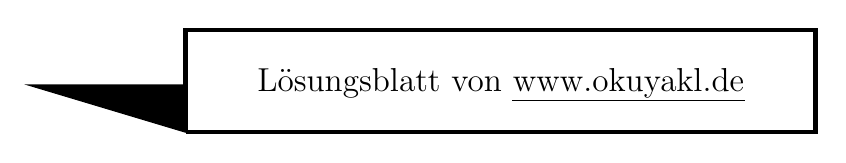
\begin{tikzpicture}(10,3)
	\draw[ultra thick](2,0) --(10,0) -- (10,1.3) --(2,1.3) -- (2,0);
	\draw[fill=black](2,0)-- (0,.6) -- (2,.6) -- (2,0);
	\node at (6,.6) {\large Lösungsblatt von \href{https://www.okuyakl.de}{www.okuyakl.de}};
\end{tikzpicture}


\section*{1. Der faule Kater und die Wärmflasche}

\begin{itemize}
	\item \( m = 2\,\text{kg} \) (2 L Wasser),  
	\( \Delta \vartheta = 60^\circ C - 20^\circ C = 40\,\text{K} \),  
	\( c = 4{,}18\,\frac{\text{kJ}}{\text{kg}\cdot\text{K}} = 4180\,\frac{\text{J}}{\text{kg}\cdot\text{K}} \)
	
	\item a)  
	\[
	Q = 4180 \cdot 2 \cdot 40 = \underline{334400\,\text{J}}\approx 0,33 \,\text{MJ}
	\]
	
	\item b) \( Q_\text{Wärme} = 80\,\% \) von 334400 J:  
	\[
	Q = 0{,}8 \cdot 334{,}400 = \underline{267520\,\text{J}}\approx 0,27 \,\text{MJ}
	\]
\end{itemize}

\hrulefill

\section*{2. Die Spaghetti-Aktion}

\begin{itemize}
	\item \( m = 0{,}5\,\text{kg} \),  
	\( \Delta \vartheta = 100^\circ C - 15^\circ C = 85\,\text{K} \)
	
	\item a)  
	\[
	Q = 4180 \cdot 0{,}5 \cdot 85 = \underline{177650\,\text{J}}\approx 0,18\, \text{MJ}
	\]
	
	\item b) Tatsächlicher Energieeinsatz bei 80 \% Wirkungsgrad:  
	\[
	Q = \frac{177{,}650}{0{,}8} = \underline{222063,\text{J}}\approx 0,22 \,\text{MJ}
	\]
\end{itemize}

\hrulefill

\section*{3. Die Badewanne für Astronauten}

\begin{itemize}
	\item \( m = 100\,\text{kg} \),  
	\( \Delta \vartheta = 20\,\text{K} \)
	
	\item a)  
	\[
	Q = 4180 \cdot 100 \cdot 20 = \underline{8360000\,\text{J}}\approx 8,4\, \text{MJ}
	\]
	
	\item b) Dauer: 10 Minuten = 600 Sekunden.  
	Pro Heizstab (1000 W) kommen 600000 J in 10 Minuten.  
	\[
	\frac{8360000}{600000} = \underline{13{,}93 \approx 14 \,\text{ Heizstäbe}}
	\]
\end{itemize}

\hrulefill

\section*{4. Die lauwarme Liebeserklärung}

\begin{itemize}
	\item \( m = 0{,}25\,\text{kg} \),  
	\( \Delta \vartheta = 35\,\text{K} \)
	
	\item a)  
	\[
	Q = 4180 \cdot 0{,}25 \cdot 35 = \underline{36575\,\text{J}}\approx 37 \,\text{kJ}
	\]
	\item b) Mit 10 \% Verlust $\Rightarrow$  90 \% = \( 0{,}9 \cdot Q_\text{real} = 36575\,\text{J} \)  
	\[
	Q_\text{real} = \frac{36575}{0{,}9} = \underline{40639\,\text{J}}\approx 41 \,\text{kJ}
	\]
\end{itemize}


\section*{5. Die heiße Schraube }

\begin{itemize}
	\item a) \( m = 0{,}3\,\text{kg} \), \( \Delta \vartheta = 160\,\text{K} \), \( c = 450 \,\frac{\text{J}}{\text{kg}\cdot\text{K}}\)
	
	\[
	Q = 450 \cdot 0{,}3 \cdot 160 = \underline{21600\,\text{J}}\approx 22 \,\text{kJ}
	\]
	
	\item b) \( m = 0{,}6\,\text{kg} \)
	
	\[
	Q = 450 \cdot 0{,}6 \cdot 160 = \underline{43200\,\text{J}}\approx 43\, \text{kJ}
	\]
\end{itemize}

\hrulefill

\section*{6. Die schmelzende Butter }

\begin{itemize}
	\item a) \( m = 0{,}25\,\text{kg} \), \( \Delta \vartheta = 34\,\text{K} \), \( c = 2100 \,\frac{\text{J}}{\text{kg}\cdot\text{K}}\)
	
	\[
	Q = 2100 \cdot 0{,}25 \cdot 34 = \underline{17850\,\text{J}}\approx 18 \,\text{kJ}
	\]
	
	\item b) \( Q = 17{,}850\,\text{J} \), \( m = 0{,}125\,\text{kg} \)
	
	\[
	\Delta \vartheta = \frac{Q}{c \cdot m} = \frac{17{,}850}{2100 \cdot 0{,}125} = \underline{68\,\text{K}}
	\]
\end{itemize}

\hrulefill

\section*{7. Der feurige Ziegelstein }

\begin{itemize}
	\item \( m = 2\,\text{kg} \), \( \Delta \vartheta = 875\,\text{K} \), \( c = 840\,\frac{\text{J}}{\text{kg}\cdot\text{K}} \)
	
	\[
	Q = 840 \cdot 2 \cdot 875 = \underline{1470000\,\text{J}}\approx 1,5 \,\text{MJ}
	\]
	
	\item b) Die Farbe beeinflusst die Absorption von Wärmestrahlung: dunkle Farben wie Rot oder Schwarz nehmen mehr Strahlung auf → schnellere Erwärmung.
\end{itemize}

\hrulefill

\section*{8. Der Käsewürfel im Toaster }

\begin{itemize}
	\item \( m = 0{,}05\,\text{kg} \), \( \Delta \vartheta = 50\,\text{K} \), \( c = 3100 \,\frac{\text{J}}{\text{kg}\cdot\text{K}}\)
	
	\[
	Q = 3100 \cdot 0{,}05 \cdot 50 = \underline{7750\,\text{J}}
	\]
	
	\item \( P = 150\,\text{W} \), also \( t = \frac{Q}{P} = \frac{7750}{150} \approx \underline{52\,\text{s}} \)
\end{itemize}

\hrulefill

\section*{9. Sauna mit Holzbank }

\begin{itemize}
	\item a) \( m = 1{,}5\,\text{kg} \), \( \Delta \vartheta = 50\,\text{K} \), \( c = 1700\,\frac{\text{J}}{\text{kg}\cdot\text{K}} \)
	
	\[
	Q = 1700 \cdot 1{,}5 \cdot 50 = \underline{127500\,\text{J}}\approx 0,13 \,\text{MJ}
	\]
	
	\item b) \( c_\text{Alu} = 900 \)
	
	\[
	Q = 900 \cdot 1{,}5 \cdot 50 = \underline{67500\,\text{J}}\approx 68\,\text{kJ}
	\]
\end{itemize}


\begin{center}
	\includegraphics[width=7 cm]{../../viecher/endcomic.pdf}
	
	Hier geht es zurück zum \href{https://www.okuyakl.de/phys/p9qcmL116/aa116.pdf}{Aufgabenblatt}
\end{center}
\end{document}

